\begin{block}{$\textsc{Bucketing-Generator}$ \& $\textsc{Random-Neighbor}$ Queries}

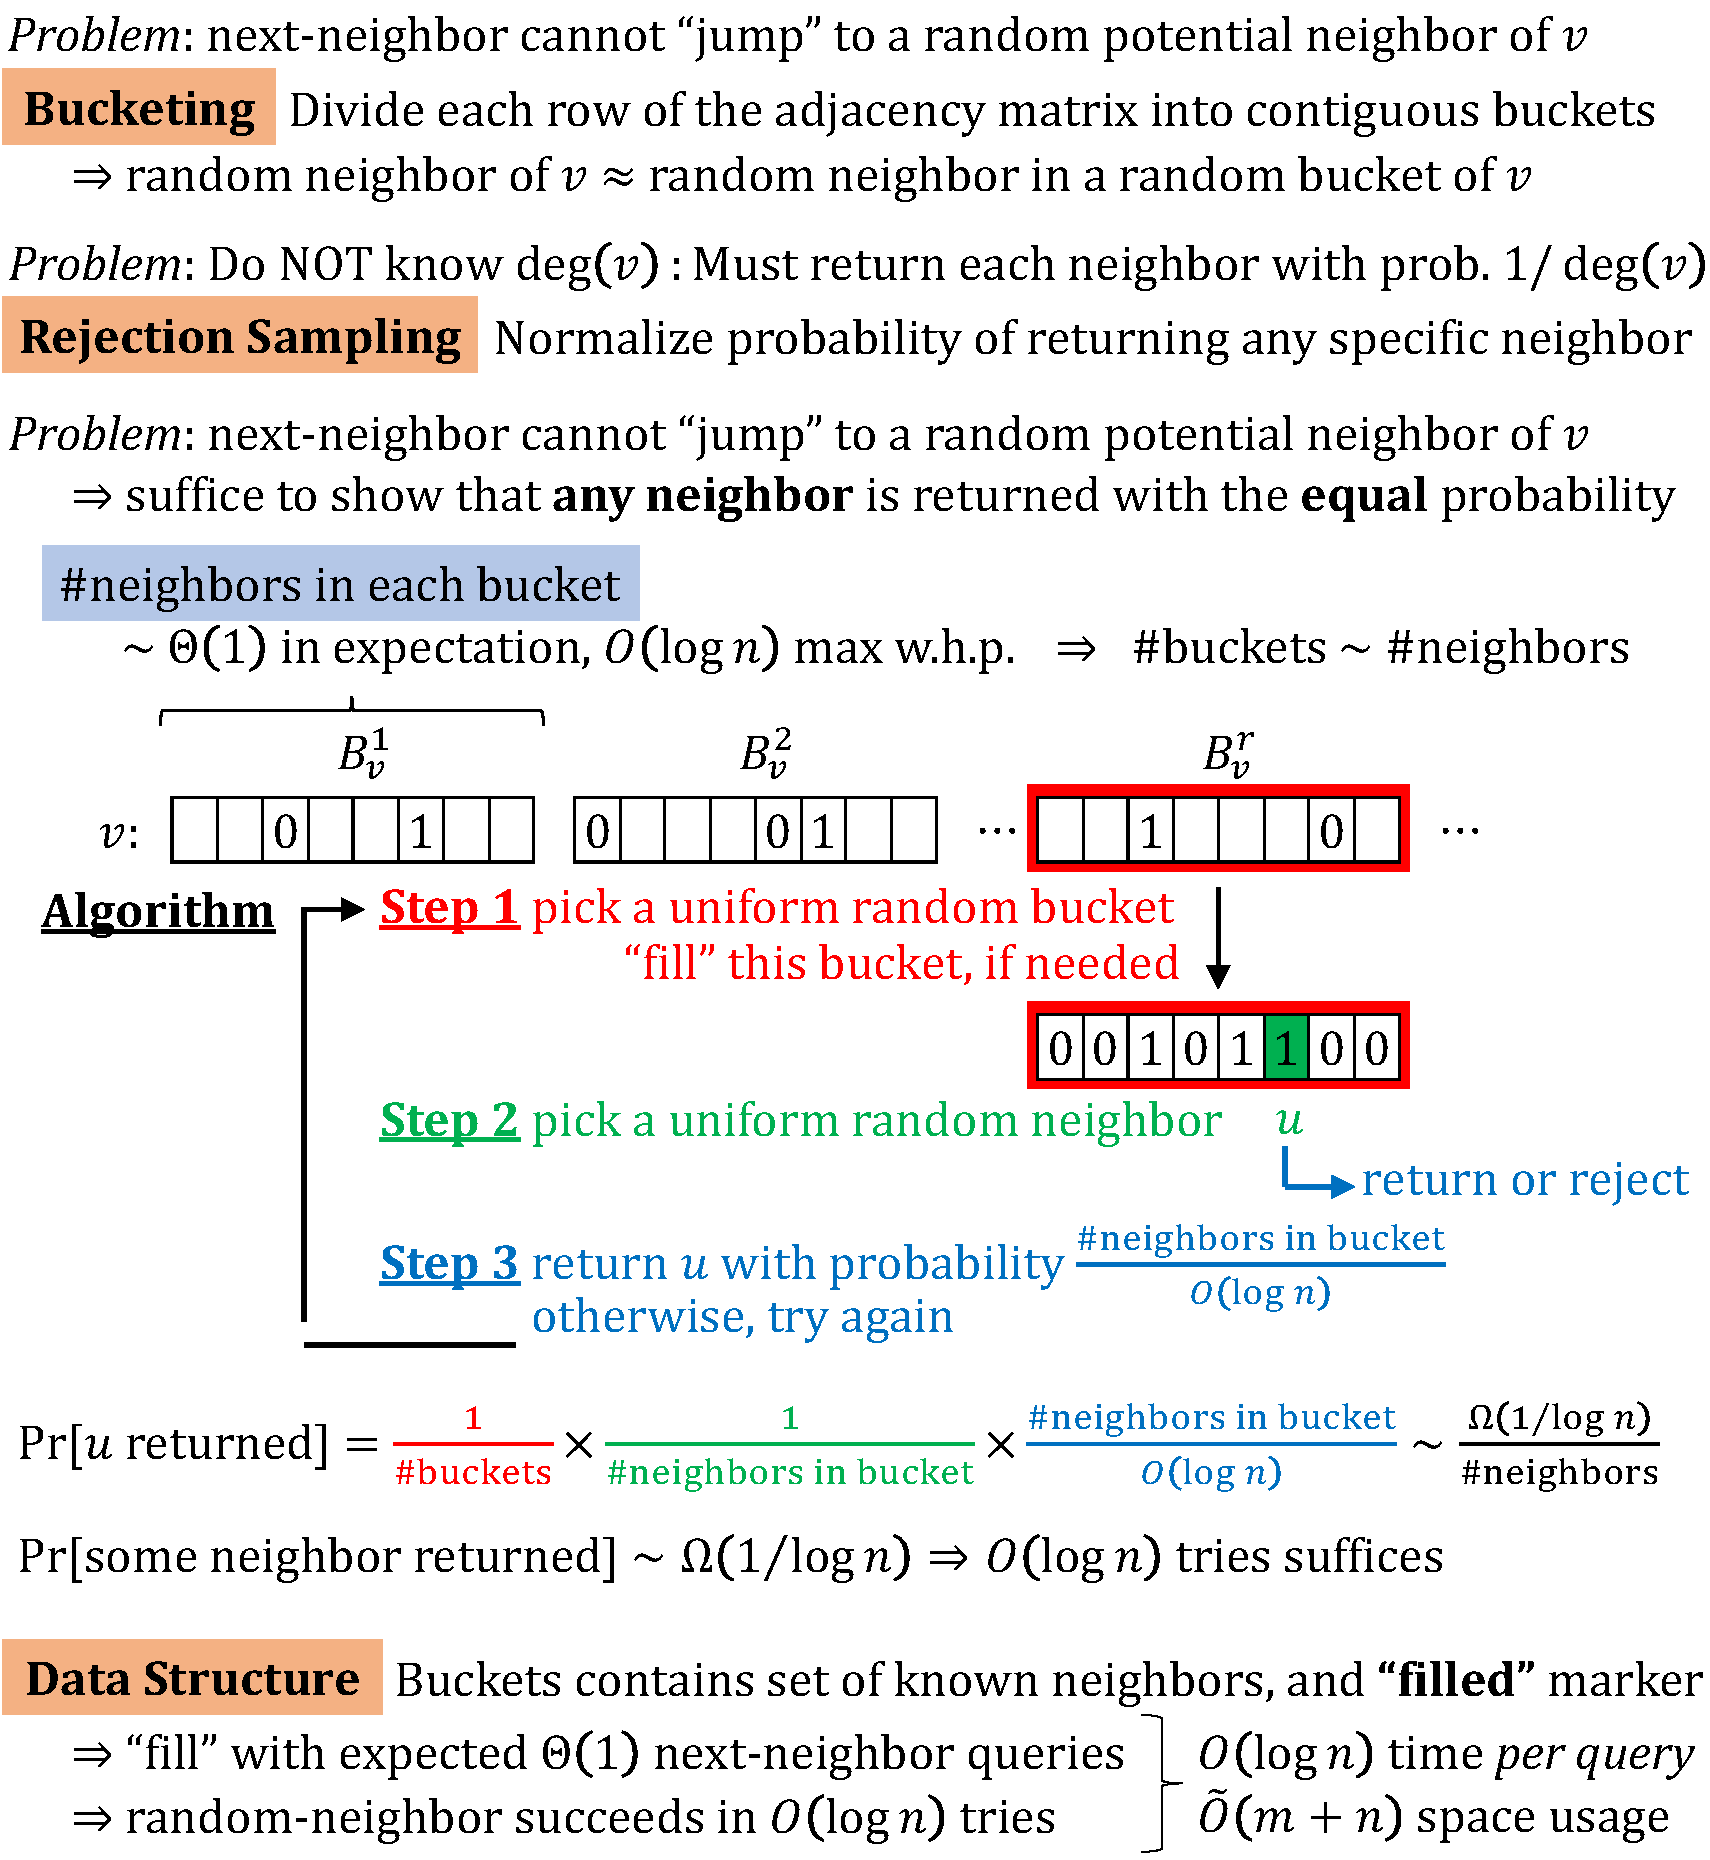
\includegraphics[clip, width=1.01\textwidth]{bucket.pdf}

%Issue: $\textsc{next-neighbor}$ can't jump to a random potential neighbor of $v$
%\begin{itemize}
    %%\item [] \textbf{Bounding the number of re-samplings:}
    %\item Divide each row of the adjacency matrix into contiguous buckets
    %\item Expected number of neighbors in a bucket is $\Theta(\log n)$
    %\item Each vertex $v$ is associated with buckets $ \langle B^v_1, B^v_2, B^v_3,\cdots\rangle$
    %\item An \textbf{unfilled} bucket may contain some indirectly exposed neighbors
    %\item A \textbf{filled} bucket will contain every possible sampled neighbor
%\end{itemize}

%%\setbeamercolor{block alerted title}{bg=Periwinkle} % Change the alert block title colors
%\begin{alertblock}{Filling the $i^{th}$ bucket $B^v_i$ of vertex $v$}
%\begin{itemize}
    %\item Use skip-sampling to produce a \textbf{potential} \emph{next-neighbor} $u$ of $v$ in $B^v_i$
    %\item Check if $(u, v)$ was set to $0$, by looking at bucket $\mathcal B$ of $u$ containing $v$
    %\item If so, re-sample. Otherwise, mark $u$ as a neighbor of $v$, and update $\mathcal B$
    %\item W.h.p, only $\mathcal O(\log^2 n)$ \textbf{potential} neighbors are generated in $B^v_i$
    %%\item With high probability, none of the buckets contain zero neighbors.
%\end{itemize}
%\end{alertblock}

\end{block}



%\vspace{-0.5in}
%%\begin{columns}[t,totalwidth=\twocolwid]

%%\begin{column}{0.49\twocolwid}

%\begin{itemize}
    %\item [] \textbf{Degree Sampling:} Sampling the degree of $v$ seems to be much harder
    %\item Sampling $deg(v)$ conditions the remaining RVs in very non-trivial ways
    %\item However, we can stil sample a random neighbor (with prob. $1/deg(v)$)
%\end{itemize}

%%\setbeamercolor{block alerted title}{bg=Periwinkle} % Change the alert block title colors
%\begin{alertblock}{$\textsc{Random-Neighbor}(v)$}
%\begin{itemize}
    %\item Choose a random bucket $\mathcal B$ of $v$. If the $\mathcal B$ is \textbf{unfilled}, fill it.
    %\item If $k$ neighbors found in $\mathcal B$, start over (reject) with probability $1-k/M$.
    %\item If accepted, return an uniformly random neighbor found in $\mathcal B$.
%\end{itemize}
%For $M = \mathcal O(\log^2 N)$, the max number of neighbors in any bucket is $<M$.
%So, the number of rejection sampling rounds is $\mathcal O(\log^2 N)$ in expectation.
%\end{alertblock}
